\section{Methodology}

This chapter describes the methodological design used to evaluate the cost of stronger access control in a smart-lock-based booking system. The evaluation follows a comparative approach: the same booking and access use case is implemented with three different access control scenarios, each representing a different security level. The scenarios are then compared using cloud cost and infrastructure resource metrics.

\subsection{High-Level Use Case}

The use case considered in this work is a booking-based access control process for music studios. A user books a studio for a specific time window and should only be able to enter the room during this valid booking period. The physical entry point is protected by a Nuki Smart Lock and keypad, while the access decision is controlled by a cloud-based backend system.

At a high level, the process consists of four steps. First, a user creates a booking for a studio. Second, the system stores the booking and associates it with a valid access period. Third, the user attempts to access the studio at the door. Fourth, the system either grants or denies access depending on the selected access control scenario. This is illustrated in Figure~\ref{fig:high_level_use_case}.

This leads to a security-cost trade-off: higher assurance can reduce the risk of unauthorized access, but it also increases infrastructure resource usage, operational complexity, and cloud cost.

\begin{figure}[H]
\centering
\resizebox{\linewidth}{!}{%
\begin{tikzpicture}[node distance=0.5cm and 0.9cm]

    \node[box] (user)    {User};
    \node[box, right=of user]    (book)    {Create Booking};
    \node[box, right=of book]    (arrive)  {Arrive at Studio};
    \node[box, right=of arrive]  (verify)  {Present Credentials};
    \node[decision, right=of verify] (check) {Valid?};
    \node[box, above right=0.3cm and 0.8cm of check, fill=green!10] (grant) {Access Granted};
    \node[box, below right=0.3cm and 0.8cm of check, fill=red!10]   (deny)  {Access Denied};

    \draw[arrow] (user)   -- (book);
    \draw[arrow] (book)   -- (arrive);
    \draw[arrow] (arrive) -- (verify);
    \draw[arrow] (verify) -- (check);
    \draw[arrow] (check)  -- node[above, font=\scriptsize]{Yes} (grant);
    \draw[arrow] (check)  -- node[below, font=\scriptsize]{No}  (deny);

\end{tikzpicture}%
}
\caption{High-level booking and access control use case.}
\label{fig:high_level_use_case}
\end{figure}

\subsection{System Architecture and Roles}

The prototype is implemented as a microservice application consisting of four Spring Boot 3.5.6 services deployed on AWS ECS Fargate and exposed via an Application Load Balancer (ALB) with path-based routing rules. All services persist data in dedicated Amazon RDS PostgreSQL 17 databases on a \texttt{db.t3.micro} instance. Table~\ref{tab:responsibilities} summarizes the main roles of the system components.

\begin{table}[H]
\centering
\caption{System roles and responsibilities}
\label{tab:responsibilities}
\begin{tabular}{p{1.2cm}p{3.2cm}p{8.0cm}}
\hline
\textbf{ID} & \textbf{Component} & \textbf{Responsibility} \\
\hline
R1 & User Service      & Manages authentication and user data. Issues JWT tokens signed with a shared HMAC-SHA256 secret and validates incoming Bearer tokens using Spring Security's JWT decoder. \\
R2 & Studio Service    & Manages studio entities, availability, and Nuki smartlock associations. \\
R3 & Booking Service   & Creates and stores bookings, including the booked studio, user, and valid time window. Upon booking creation, it synchronously calls the Access Service to initialize the access permission. \\
R4 & Access Service    & Implements the scenario-specific access control logic. This is the primary measurement subject in this evaluation. \\
R5 & Nuki Smart Lock   & Provides the physical access mechanism. The lock executes time-limited keypad codes registered by the Access Service via the Nuki Web API. \\
\hline
\end{tabular}
\end{table}

The Access Service (R4) is deployed as a single ECS Fargate task with 0.25 vCPU and 512\,MB memory. The active security scenario is selected at startup via the \texttt{FA\_LEVEL} environment variable, which activates the corresponding implementation through Spring Boot's \texttt{@ConditionalOnProperty} mechanism. All three implementations share a common abstract base class and differ only in the access-time flow.

For face verification (Cases 2 and 3), the system relies on a pre-built Amazon Rekognition face collection. User face enrollment is handled by a separate service in a distinct repository, implementing the following pipeline: a user photo is uploaded to Amazon S3, which triggers an AWS Lambda function that invokes the Rekognition \texttt{IndexFaces} API and stores the resulting \texttt{FaceId} and user identity in Amazon DynamoDB. This enrollment pipeline runs once per user and is independent of the per-access-attempt flow evaluated in this work.

\subsection{Access Control Scenarios}

Three access control scenarios are implemented and compared. They represent increasing security levels and differ in how much verification is performed at the moment of access.

\textbf{Case 1: Single-Factor Access (1FA).}
At booking creation, the Access Service generates a six-digit PIN, encrypts and stores it in PostgreSQL, and immediately registers a time-limited keypad code on the Nuki lock via the Nuki Web API. At access time, the user enters this PIN directly at the Nuki keypad without any further backend interaction. The sole authentication factor is knowledge of the booking code. No AWS managed services are invoked per access attempt.

\textbf{Case 2: Two-Factor Access (2FA).}
At booking creation, the Access Service stores the encrypted PIN in the database without registering a Nuki code. At access time, the following steps are performed: (1) the user submits the booking PIN on a separate dashboard, which the Access Service validates against a stored SHA-256 hash. (2) The user captures a selfie, which the Access Service passes in-memory to the Amazon Rekognition API against the pre-built face collection. (3) Upon successful biometric verification, the Access Service generates a new Nuki code, registers it via the Nuki Web API, and returns it to the application for display. The two authentication factors are knowledge of the booking code and biometric identity.

\textbf{Case 3: Three-Factor Access (3FA).}
Case 3 is identical to Case 2 in all steps except the delivery of the Nuki code. Instead of returning the code to the application for display, the Access Service invokes Amazon SES to send the code to the user's registered email address. The code is not shown in the application. The three authentication factors are knowledge of the booking code, biometric identity, and possession of the registered email account.

\begin{figure}[H]
\centering
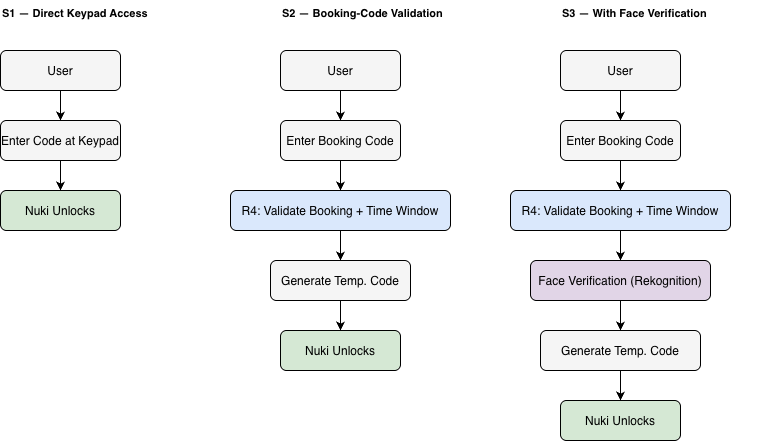
\includegraphics[width=\linewidth]{fig/scenarios.png}
\caption{Comparison of the three access control scenarios with mapped evaluation metrics.}
\label{fig:scenario_comparison}
\end{figure}

\subsection{Evaluation Metrics}

The evaluation uses three metrics to quantify the cost of stronger access control. The metrics focus on the Access Service because it contains the scenario-specific access logic. The User Service, Studio Service, and Booking Service behave identically across all scenarios and are excluded from metric collection accordingly.

\begin{itemize}
    \item \textbf{M1: Cost per Access Attempt.}
    The average variable AWS service cost per access attempt in each scenario. Calculated by dividing the total scenario-related variable cloud cost by the number of executed access attempts. Fixed infrastructure costs (ECS Fargate, RDS, VPC, ALB) are excluded as they are invariant across scenarios.

    \item \textbf{M2: Average CPU Utilization.}
    The average CPU utilization of the Access Service during the test window, reported as a percentage of the allocated 0.25 vCPU, collected via Amazon CloudWatch Container Insights at one-minute granularity.

    \item \textbf{M3: Average Memory Utilization.}
    The average memory utilization of the Access Service during the test window, reported as a percentage of the allocated 512\,MB, collected via Amazon CloudWatch Container Insights at one-minute granularity.
\end{itemize}

The cost per access attempt (M1) is calculated as follows:

\begin{equation}
\text{M1} = \frac{\text{Total Scenario-Related Variable AWS Cost}}{\text{Number of Access Attempts}}
\end{equation}

\subsection{Measurement and Data Collection}

Variable cost data is derived from AWS public pricing as of June 2026, applied to the exact number of external service invocations per access attempt. At access time, Case 2 invokes one Rekognition \texttt{SearchFacesByImage} call (\$0.001 per image). Case 3 additionally invokes one Amazon SES send (\$0.0001 per message). Case 1 invokes no AWS managed services at access time. The face enrollment pipeline (S3, Lambda, \texttt{IndexFaces}, DynamoDB) is a one-time per-user operation and is excluded from per-attempt cost calculations. The Nuki Web API is billed externally to AWS and is also excluded.

Fixed infrastructure costs (ECS Fargate, RDS, VPC, ALB) are treated as a shared baseline invariant across all three scenarios and are reported separately for reference.

CPU and memory utilization metrics are collected via Amazon CloudWatch Container Insights for the Access Service ECS task, using one-minute average statistics. Because all three scenarios run on identical task configurations (0.25 vCPU, 512\,MB), the reported percentages are directly comparable without normalization.

\subsection{Test Execution}

Each scenario is executed under identical infrastructure conditions. The same ECS task configuration, RDS instance class, ALB listener rules, and CloudWatch monitoring setup are applied consistently. No auto-scaling policies are active during the test window.

For each scenario, 20 bookings and 20 corresponding access attempts are executed sequentially via the application under controlled conditions. All three runs are conducted on 2026-06-18 with the \texttt{FA\_LEVEL} environment variable set to \texttt{1}, \texttt{2}, and \texttt{3} for Case 1, Case 2, and Case 3, followed by an ECS force redeployment between scenarios.

After execution, data is grouped by scenario and evaluated against M1, M2, and M3.
